\documentclass[conference]{IEEEtran}
\IEEEoverridecommandlockouts
% The preceding line is only needed to identify funding in the first footnote. If that is unneeded, please comment it out.
%\usepackage{cite}
\usepackage[portuges,brazil,english]{babel}
\usepackage[utf8]{inputenc}
\usepackage{hyperref}
\usepackage{amsmath,amssymb,amsfonts}
\usepackage{amsmath}
\usepackage{algorithm}
\usepackage{algorithmic}
\usepackage{graphicx}
\usepackage{textcomp}
\DeclareUnicodeCharacter{00A0}{ }
\def\BibTeX{{\rm B\kern-.05em{\sc i\kern-.025em b}\kern-.08em
    T\kern-.1667em\lower.7ex\hbox{E}\kern-.125emX}}
\begin{document}

\title{Algoritmos genéticos aplicados ao Tetris}

\author{\IEEEauthorblockN{André Almeida}
\IEEEauthorblockA{
RA: 164047}
\and
\IEEEauthorblockN{Igor Torrente}
\IEEEauthorblockA{
RA: 169820}
\and
\IEEEauthorblockN{Lucas Cunha}
\IEEEauthorblockA{
RA: 172655}
\and
\IEEEauthorblockN{João Spuri}
\IEEEauthorblockA{
RA: 155943}}


\maketitle

\section{Resumo}
Nesse projeto, foi proposta e experimentada uma abordagem para a criação de um algoritmo que consiga fazer jogadas no jogo eletrônico \textit{Tetris}, obtendo uma pontuação compatível com a esperada por humanos. Para tal, foram utilizadas técnicas de algoritmos genéticos aplicadas em redes neurais artificiais.

\section{Introdução}

\subsection{Tetris}
\subsubsection{O jogo}
Tetris é um jogo eletrônico criado em 1984 pelo matemático soviético Alexey Pazhitnov, tendo obtido grande popularidade principalmente nas plataformas \textit{Atari  ST} e no \textit{Nintendo Entertainment System} \cite{b1}. Até hoje, já foram vendidas mais de 50 milhões de cópias mundialmente. O jogo é do gênero \textit{puzzle}, onde o jogador precisa resolver algum tipo de quebra-cabeça.

No Tetris, o "tabuleiro" do jogo é formado por uma malha de 22\textit{x}10 quadrados (com as duas linhas do topo ocultas ao jogador), onde o jogador deve ir encaixando as peças (os "Tetraminós") que caem verticalmente no tabuleiro em uma sequência aleatória. Existem 7 tipos de Tetraminós, cada um formato distinto. O objetivo do jogador é manipular essas peças, movendo-as horizontalmente e girando-as de forma a criar uma linha horizontal no tabuleiro sem espaços vazios. Quando uma linha assim é completa, ela é destruída, as peças acima dela "caem" uma linha para baixo e o jogador pontua.

Conforme as linhas vão sendo limpas, o jogador avança entre níveis mais difíceis. A cada nível, as peças caem mais rapidamente, exigindo um tempo de resposta cada vez maior do jogador. O jogo acaba quando alguma peça, por falta de espaço no tabuleiro, fica com alguma parte posicionada fora do tabuleiro (acima da linha 22).

\begin{center}
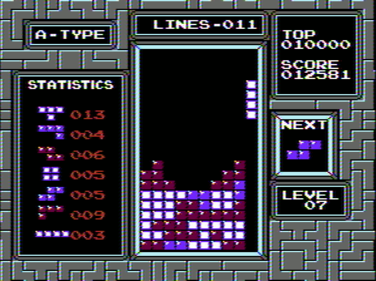
\includegraphics[scale=0.5]{tetris_nes.png}\\

\textbf{Figura 1:} \textit{captura de tela da versão} NES \textit{do jogo}
\end{center}

\subsubsection{Complexidade computacional}
Foi provado \cite{b2} que em uma versão de Tetris onde o jogador já conhece toda a sequência de peças que virão, os seguinte objetivos são problemas NP-Completos:
\begin{itemize}
\item Maximizar o número de linhas limpas enquanto joga com a sequência dada;

\item Maximizar o número de peças colocadas antes de completar uma linha;

\item Maximizar o número de pontuações simultâneas de quatro linhas;

\item Minimizar a altura da última peça colocada em uma sequência.

\end{itemize}

Com exceção do terceiro, todos esses objetivos também são difíceis de serem aproximados. 

\subsection{Algoritmos genéticos}
Um algoritmo genético é uma técnica para encontrar uma solução ideal ou próxima à ideal para um problema computacional, com inspirações nas teorias darwinistas de evolução dos seres vivos. As iterações do algoritmo são sobre as gerações, onde uma geração é um conjuto de indivíduos e indivíduos são funções/modelos. Em síntese, um algoritmo genético funciona da seguinte maneira \cite{b3}:

\begin{enumerate}
\item Os parâmetros dos indivíduos da primeira geração são gerados randomicamente;

\item Algum tipo de função de custo é aplicada para avaliar cada indivíduo. Essa função é usada para determinar o sucesso dos indivíduos;

\item Alguma porcentagem dos melhores indivíduos (segundo seus resultados do item anterior) é escolhida.

\item Os indivíduos escolhidos no item anterior serão os "pais" da nova geração. A partir deles, combinações e mutações irão gerar os outros indivíduos da nova geração.

\item Repita os passos 2-4 até alguma condição de parada for atingida. Quando isso acontecer retorna o melhor indivíduo da última geração.

\end{enumerate}


\subsection{Redes neurais artificiais}
Rede neural artificial é uma coleção de unidades chamadas neurônios que são interligados entre si com uma ordem (camadas), com inspiração biológica no funcionamento do cérebro dos animais. Cada neurônio de uma camada se liga a todos os neurônios da anterior (se não for a camada de entrada) e da posterior (se não for a camada de saída). Cada neurônio é ativado de acordo com uma função de ativação, os parâmetros dessa função de ativação são as saídas dos neurônios anteriores multiplicados por um peso nas arestas que conectam estes neurônios. Nos neurônios de entrada são inseridos metadados e nas funções de saída algum tipo de resposta ou classificação \cite{b4}.\\

\subsection{Aprendizado de máquina para jogos eletrônicos}
Aprendizado de máquinas aplicado em jogos eletrônicos vem sendo estudado pela academia como forma de avaliar a capacidade da máquina de executar tão bem quantas tarefas complexas, como é o caso de jogar videogames. Um estudo em destaque é o caso do AlphaGo, uma inteligência artificial que usa técnicas de aprendizado profundo e conseguiu vencer o campeão mundial do jogo Go \cite{b5}. Alguns desses estudos utilizam a técnica de algortimos genéticos para encontrar um modelo computacional adequado para o jogo, e acabaram gerando modelos que são compatíveis com o desempenho de jogadores reais, em jogos como Snake \cite{b6} e Counter-Strike \cite{b7}. Nesses jogos, parâmetros como pontuação do jogador e desempenho estratégico são usados como função de custo para treinar o algoritmo.

\subsection{Trabalhos relacionados}
Em \cite{b8}, o autor cria uma rede neural para jogar Tetris, usando algoritmos genéticos para otimizar os pesos dos neurônios (substituindo o \textit{backpropagation}). O jogador pontua ao descer peças no tabuleiro e completar linhas. A função de custo é composta por:

\begin{itemize}
\item número de linhas completadas;
\item altura máxima, altura acumulada;
\item altura relativa, buracos das linhas;
\item completude do tabuleiro.
\end{itemize}

Durante o jogo, a cada nova peça, todas as jogadas possíveis são testadas e a que retornar a melhor pontuação (seguindo as heurísticas acima) é executada.

No trabalho \cite{b9}, o autor utiliza uma função com as heurísticas: 

\begin{itemize}
\item altura agregada;
\item linhas completadas;
\item buracos;
\item diferença de alturas vizinhas.
\end{itemize}

Novamente, todas as jogadas possíveis são testadas e a que retornar o maior valor é executada. A função utilizada é a soma do produto das heurísticas com uma variável de valor inicialmente desconhecido. Os pesos de cada uma das heurísticas foi determinado usando algoritmos genéticos. 

No artigo \cite{b10}, as autoras utilizam uma metodologia semelhante à vista em \cite{b9}, porém com as seguintes heurísticas: 

\begin{itemize}
\item maior pilha; 
\item buracos;
\item buracos conectados;
\item linhas removidas;
\item diferença de altitude;
\item profundidade máxima;
\item soma dos vales;
\item altura do último tetraminó; 
\item número de células ocupadas;
\item número de células ocupadas por coluna;
\item soma de transições ocupadas/desocupadas horizontalmente e verticalmente. 
\end{itemize}

A função de custo é dado por $\sum_{i=1}^n  w_{i}|r_{i}(b)-d_{i} | ^{e_{i}}$, onde $r_{i}(b)$ é o valor retornado por cada uma das heurísticas e os valores de $w_i$, $d_i$ e $e_i$ foram descobertos utilizando algoritmos genéticos.

\subsection{Tecnologias empregadas}
Para treinamento das redes neurais, foi utilizada a versão com OpenCL\cite{b11} do Torch\cite{b12}, um framework de computação cientifica para LuaJIT\cite{b13}. Reutilizamos o Tetris feito em \cite{b14}, devido a simplicidade (o jogo é executado em um emulador de terminal), boa documentação e porque foi escrito em Lua, facilitando a integração dos dois programas e a modificação do jogo.

\subsection{Abordando o problema}
A partir disso, decidimos explorar o uso de redes neurais artificias combinadas com algoritmos genéticos com entradas/saídas diferentes dos outros trabalhos citados para chegarmos em resultados melhores.

\section{Metodologia}
Utilizamos redes neurais artificiais para fazer as jogadas automaticamentes. Como em \cite{b8}, substituímos a parte do \textit{backpropagation} pelo algoritmo genético. Nosso \textit{crossover}, pega aleatoriamente os dez melhores indivíduos de cada população para cruzamento. Além disso, casa peso dos neurônios tem 30\% de chance de ter seu valor alterado pela soma de algum valor aleatório, que seria nossa mutação.   Porém, diferentemente dos outros trabalhos, a saída da nossa rede é composta por 14 neurônios: qual das 10 colunas a peça deve ser posicionada e em qual das 4 rotações possíveis. Dessa forma, pretendíamos reduzir o custo computacional de simular todas as jogadas possíveis e ser uma saída mais próxima do que um jogador humano faria. A entrada da nossa rede era, inicialmente, 221 neurônios representando o tabuleiro de 22x10 linearizado, onde um neurônio ativado indicava que havia alguma peça ocupando aquela posição e um neurônio para indicar qual o \textit{id} da peça a ser colocada. Essa entrada tinha como objetivo ser mais parecida com o que um humano recebe ao olhar para o tabuleiro.

Para comparar o desempenho do modelo com jogadores humanos, coletamos dados de 50 jogos: pedimos que 10 pessoas jogassem 5 vezes a mesma implementação de Tetris escolhida para nossos experimentos. Com isso, obtivemos que, antes de perder o jogo, um humano chega em média ao level 5, fazendo 40 linhas e um score de 70.

Tentamos várias funções de custos, iniciando como somente o número de linhas limpadas na média de dez jogos e a pontuação padrão do Tetris como critério de desempate, porém logo percebemos que essa função insentivava as redes a somente espalharem as peças mais do que realmente limparem linhas.

Dessa forma uma nova função de custo foi formulada, na qual quanto mais "fundo" a peça estivesse no tabuleiro, mais pontos ela valia. Porém, se a peça fosse colocada a cima da metade do tabuleiro, quanto mais alta ela fosse colocada, mais ele era penalizado. Neste caso tivemos problemas com pontuações negativas, o que levava em alguns casos a escolha errada das melhores redes.

Finalmete, a função escolhida foi a qual cada peça vale mais pontos se colocada mais no fundo, porém essa pontuação é então dividida pela altura da maior torre atual no jogo, o que leva a rede a espalhar mais as suas peças, mas também incentiva ela a construir torres menores, o que por consequência a limpar mais linhas.

Ao ordenar os indivíduos para a escolha do crossover, primeiro eles eram ordenados pelo número de linhas completadas e, em cada conjunto de indivíduos que completaram a mesma linha, eram ordenados pela pontuação. Dessa forma, a função de custo deveria escolher os indivíduos que mais inserissem peças ao fundo do tabuleiro, causando assim uma maior alocação de peças na base e, consequentemente, mais linhas concluídas e mais distante do topo (onde o jogo é finalizado).

Entretanto para a versão final da função de custo, passamos a ordenar as redes somente pela pontuação, pois percebemos que a ordenação por linhas causava a algumas boas redes que fossem eliminadas por má sorte.

Modificamos o código-fonte do jogo de forma que ele posicionasse as peças na coluna indicada e com a rotação indicada. A cada peça colocada, a rede recebia a entrada do tabuleiro e retornava uma nova configuração de coluna/rotação. Cada rede jogava o jogo até perder 10 vezes, e cada geração continha 10 indivíduos. Ao final dos 100 jogos, o crossover era utilizado para gerar a próxima geração.

A partir disto, fizemos experimentos e conforme os resultados, fazíamos as modificações que julgávamos necessárias para melhorar a precisão de nossos modelos.

\section{Experimentos e Resultados}
No nosso primeiro teste, utilizamos o jogo de Tetris com todas as peças do jogo e uma variedade de configurações de rede neural (mudando o número de camadas, neurônios por camadas e função de ativação). Nenhuma rede, mesmo após 200 gerações evolutivas, conseguia completar mais de uma linha por jogo nem demonstrar algum avanço. 


\begin{center}
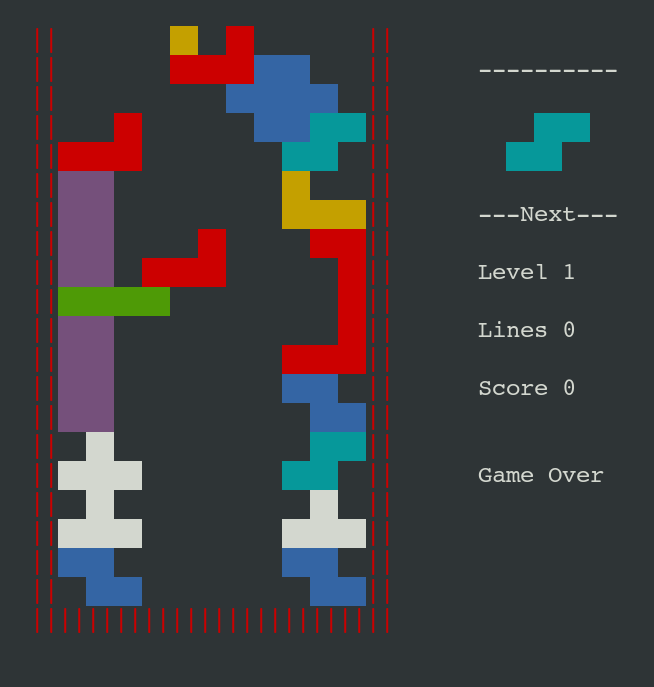
\includegraphics[scale=0.2]{tetris_lose.png}\\

\textbf{Figura 2:} \textit{Amostra da rede jogando Tetris nos primeiros experimentos}
\end{center}

Para testar a viabilidade do modelo, de forma a verificarmos de o modelo funcionaria em outras condições, mudamos o jogo para um modelo mais simples, com apenas peças de 1x1 e um tabuleiro de 10x10.

\begin{center}
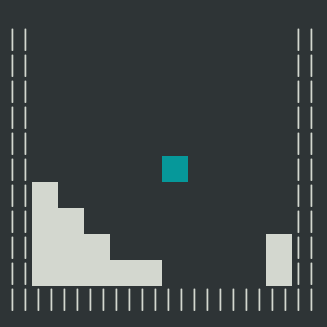
\includegraphics[scale=0.3]{tetris_simples.png}\\

\textbf{Figura 3:} \textit{Primeiro Tetris simplificado utilizado nos experimentos}
\end{center}

A melhor configuração de rede neural obtida nesse cenário foi uma rede com três camadas. A camada de entrada original foi modificada para uma com 22 neurônios:  

\begin{itemize}
\item 1 com um identificador da peça;
\item 10 com a altura de cada coluna;
\item 9 com a diferença de altura entre cada par de colunas adjacentes;
\item 1 com a maior diferença entre alturas.
\end{itemize}

A camada oculta contem 100 neurônios. A saída da rede, com 14 neurônios, indica qual das 10 colunas a peça deve ser colocada e qual a rotação dela. Depois de 12 gerações, a rede conseguiu jogar o jogo "infinitamente". Ele completava linhas sequencialmente, da mesma forma, sem fim. Um fato curioso nessa etapa do treinamento foi que a rede se aproveitou de um \textit{bug} que permitia completar linhas com muitos menos movimentos, que não era conhecido pelos desenvolvedores. Após corrigir o \textit{bug}, a rede foi retreinada e o jogo obteve o mesmo resultado de jogar infinitamente na geração 39.

A partir deste cenário, utilizamos \textit{transfer learning}. Esse conceito é utilizado em redes neurais, como forma de reaproveitar alguma parte de uma neural já treinada para outro problema parecido. Mudamos o jogo para uma outra peça, de 2x1.

\begin{center}
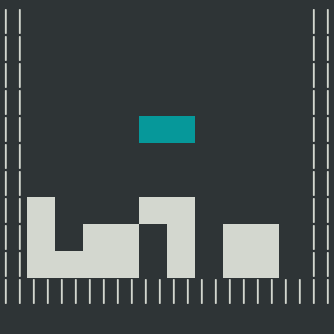
\includegraphics[scale=0.3]{tetris_simples2.png}\\

\textbf{Figura 4:} \textit{Segundo Tetris simplificado}
\end{center}

Utilizando a mesma rede que conseguia ganhar no Tetris anterior, testamos nesse novo modelo. O \textit{transfer learning} funcionou e na próxima geração a rede já conseguia completar as linhas sem fim.

Contudo, a rede novamente não conseguia jogar com modelos mais complexos a partir da rede treinada nos modelos anteriores. Ao inserirmos ambas as formas, 1x1 e 2x1, a rede não conseguia avançar e novamente limpava apenas uma linha por jogo na média. Para tentar contorna esse problema, fizemos novamente um teste com apenas uma peça, mas, dessa vez, uma mais complexa. Essa nova peça é uma "combinação" das duas peças anteriores, em um formato de \textit{L}. Contudo, a rede tentava aplicar as mesmas técnicas de antes, sem explorar as rotações ou fazendo-as de forma sem sentido. Em um jogo que precisava mais do que apenas lógica para o posicionamento, mas também lógica para rotação, a rede não obteve sucesso.

\begin{center}
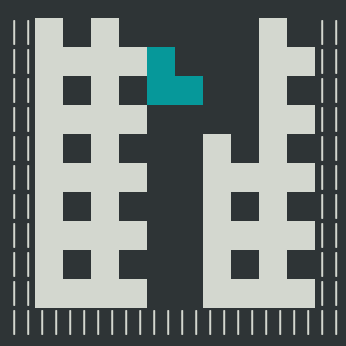
\includegraphics[scale=0.3]{tetris_lose2.png}\\

\textbf{Figura 5:} \textit{Rede jogando o quarto Tetris simplificado proposto}
\end{center}

Ao analisarmos a saída da rede, constatamos que as redes que eram bem sucedidas nas versões simplificadas faziam apenas dois movimentos, usando apenas duas das dez posições disponíveis. A rede jogava todas as peças para a coluna mais à esquerda, depois para a mais a direita e, quando ambos lados estiverem concluídos, a rede posiciona uma peça na coluna central, limpando uma linha. Isso é possível porque, no jogo, existe um sistema de colisão. Quando uma peça tenta atingir uma posição já ocupada do tabuleiro, ela não consegue avançar lateralmente. Dessa forma, a rede consegue completar duas metades do tabuleiro apenas ordenando que as peças vão para a posição mais remota possível.

\begin{center}
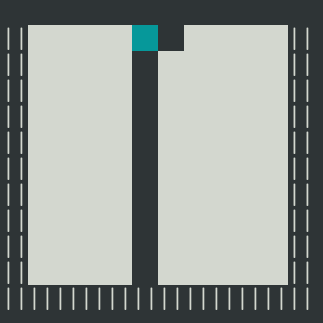
\includegraphics[scale=0.3]{tetris_win.png}\\

\textbf{Figura 6:} \textit{Rede prestes a limpar uma linha seguindo seu algoritmo}
\end{center}


\section{Conclusão}
Segundo os resultados dos nossos experimentos, a rede falhou em aprender a jogar Tetris. Apesar de conseguir jogar jogos simplificados (com apenas uma peça), ela não posiciona as peças conforme as informações retirados do tabuleiro, apenas segue uma ordem de passos que irá obter sucesso, sem depender de dados do tabuleiro. Jogos com mais de uma peça não são determinísticos, já que as peças vem de forma aleatória. Nesse cenário, um algoritmo como o executado pela rede não funciona, já que peças diferentes requerem respostas diferentes. Já em um jogo com apenas uma peça, todos os passos de sucesso são determinísticos, já que a mesma peça virá sempre. Devido as muitas variações que os jogos não determinísticos oferecem, durante o treinamento dos indivíduos da população (as redes), eles, na prática, nunca encontravam o mesmo jogo, o que pode ser um fator que dificultava o aprendizado. A abordagem de simular todas as jogadas possíveis e fazer a que tem o melhor desempenho segundo a função de custo provavelmente contorna este problema, apesar de ser contrário a nossa proposta de resolução do problema. 

A métrica utilizada para determinar o sucesso de nosso modelo (comparar com resultados humanos) não fez muito sentido na prática, pois, pelos resultados obtidos, uma rede que aprenda a jogar jogo bem provavelmente não irá cometer erros e irá jogar infinitamente, até atingir a pontuação máxima permitida no jogo.


\section{Estudos futuros}
Para melhorar os resultados de nossa abordagem, serão necessários novos estudos em relação a nossa rede. Uma das alternativas a ser testada é o uso de redes convulacionais \cite{b15}. Esse tipo de rede é utilizado principalmente com problemas relacionados à imagens, porque ela mantem informações importantes da localização entre pixels. Dessa forma, a rede não recebe apenas a matriz de pixels linearizada, mas consegue criar uma relação entre os pixels vizinhos. Isso é importante para o tabuleiro do jogo, já que pontos com/sem peça tem mais sentido sabendo as informações das casas vizinhas.

Também devem ser testados novas escolhas de funções de custo, já que em nosso trabalho focamos na função \textit{sigmoid}.

\section{Código e dados}
Todo o código do experimento pode ser encontrado em:\\
 \texttt{\url{https://github.com/andrealmeid/AutoTetris}}

\begin{thebibliography}{00}

\bibitem{b1} \texttt{ \url{http://www.atarihq.com/tsr/special/tetrishist.html}}

\bibitem{b2} Demaine, E. D., Hohenberger, S., \& Liben-Nowell, D. (2003, July). Tetris is hard, even to approximate. In COCOON (pp. 351-363).

\bibitem{b3} Goldberg, D. E. (1989). Genetic Algorithms in Search, Optimization, and Machine Learning.

\bibitem{b4}  Geron, A. (2017). \textit{Hands-on machine learning with Scikit-Learn and TensorFlow: concepts, tools, and techniques to build intelligent systems.}

\bibitem{b5} Silver, D., Schrittwieser, J., Simonyan, K., Antonoglou, I., Huang, A., Guez, A., ... \& Chen, Y. (2017). Mastering the game of go without human knowledge. Nature, 550(7676), 354-359.

\bibitem{b6} Yeh, J. F., Su, P. H., Huang, S. H., \& Chiang, T. C. (2016, November). Snake game AI: Movement rating functions and evolutionary algorithm-based optimization. In Technologies and Applications of Artificial Intelligence (TAAI), 2016 Conference on (pp. 256-261). IEEE.

\bibitem{b7} Cole, N., Louis, S. J., \& Miles, C. (2004, June). Using a genetic algorithm to tune first-person shooter bots. In Evolutionary Computation, 2004. CEC2004. Congress on (Vol. 1, pp. 139-145). IEEE.

\bibitem{b8} \texttt{\url{https://github.com/llSourcell/How_to_make_an_evolutionary_tetris_bot}}

\bibitem{b9} \texttt{ \url{https://codemyroad.wordpress.com/2013/04/14/tetris-ai-the-near-perfect-player/}}

\bibitem{b10} Böhm, N., Kókai, G., \& Mandl, S. (2005). An evolutionary approach to tetris. In The Sixth Metaheuristics International Conference (MIC2005) (p. 5).

\bibitem{b11} \texttt{\url{https://www.khronos.org/opencl/}}

\bibitem{b12} \texttt{\url{http://torch.ch/}}

\bibitem{b13} \texttt{\url{http://luajit.org/luajit.html}}

\bibitem{b14} \texttt{\url{https://github.com/tylerneylon/termtris}}

\bibitem{b15} LeCun, Y. (2015). LeNet-5, convolutional neural networks. URL: http://yann. lecun. com/exdb/lenet.

\end{thebibliography}

\end{document}
